
% vim: set ts=4 sw=4 tw=80 noexpandtab:
%******************************************************************************%
%                                                                              %
%                   FirstDay.tex                                               %
%                   Made by: 42 staff                                          %
%                                                                              %
%******************************************************************************%

\documentclass{42-en}

%******************************************************************************%
%                                                                              %
%                                   Prologue                                   %
%                                                                              %
%******************************************************************************%

\begin{document}

\title{HackHighSchool First Day}
\subtitle{Learn to 42}

\member {Kai}{kai@42.us.org}

\summary
{
The first day we are just going to practice some command line navigation, and most importantly learn how to do peer-corrections.

Have fun! It's not a serious day.
}

\maketitle

\tableofcontents

%Initialisation des headers d'exercices

%******************************************************************************%
%                                                                              %
%                                Preamble                                      %
%                                                                              %
%******************************************************************************%

\chapter{Preamble}

42 is about face to face, self-directed, peer-to-peer learning.

\begin{enumerate}

\item Face to face: humans are all social creatures, we all like to meet and know each other. Even if you are not sure how you feel about humans in large groups, being part of group can be a really powerful source of mental health and life satisfaction. Make some friends. You are not alone here :)

\item Self-directed: you will meet some older mentors here, who are 42 cadets that have volunteered to help you learn. But they are not instructors. In fact they will all be learning the same topics as you by your side. We learn by reading official documentation, tutorials, articles, and Q\&A forums. As soon as we get a clue, we run some code to see how it works. That's why this is free: it's like studying on your own, but with supportive peers all around.

\item Peer-to-peer: The more we share information and knowledge with each other, the stronger pool of talent we have to build useful applications. At 42 you will grade each others' projects face to face. Be courteous and rigorous. Give constructive feedback so that your peers do not hate you but do learn to code better than ever before.

\end{enumerate}

\startexercices


%******************************************************************************%
%                                                                              %
%                                    Goals                                     %
%                                                                              %
%******************************************************************************%

\chapter{Goals}

\begin{itemize}

	\item Start using the Slack for communications with mentors and other students.

	\item Start using intra.42.fr and explore the site.

	\item Learn how to open your correction slots and sign up for corrections.

	\item Get your programming environment set up with a text editor and terminal.

	\item Learn how to navigate the terminal, and become familiar with the text editors built into the terminal.

	\item Correct two fellow students on the First Day project and be corrected by two others.

	\hint{You WILL turn in your work today! It's only a warmup exercise, but you must practice grading each other as well!}

\end{itemize}

%******************************************************************************%
%                                                                              %
%                                        Slack                                 %
%                                                                              %
%******************************************************************************%

\chapter{Slack}

Slack is messaging platform designed for companies and communities. It's useful because we can:
\begin{itemize}

	\item Direct message people
	\item Add Slack to smartphones so messages show up like text messages
	\item Choose times of day when you are "offline" and messages are muted
	\item Create public and private groups for projects and teams
	\item Search the directory for someone you met
	\item Add chatbots that provide helpful answers automatically.

\end{itemize}

Create an account on h2s42.slack.com using the @student.42.us.org email address that displays on your Intra page. It is an email alias that will forward to the email you signed up with. It's helpful to add Slack to your phone too and enable notifications.

\hint{Make sure your account includes enough of your name that others can identify who you are.}

\hint{Add your cell phone number if you are comfortable sharing it - that way people can get in touch when it's their turn to grade your projects or vice versa.}

%******************************************************************************%
%                                                                              %
%                                      Intra                                   %
%                                                                              %
%******************************************************************************%

\chapter{Intra}

\begin{itemize}

	\item Go to intra.42.fr. Sign in with the username and password that came to your email, the one you logged into the computer with.

	\item The first page is your profile page. A few things to notice:
	\begin{itemize}
		\item Your level meter, starting at 0.0\%. As you turn in projects and have them approved by your peers you will level up! If you reach a high level you will be eligible to take our month-long C programming curriculum in the summer.
		\item Your "Correction Points" in the top left. At 42, there is a correction point economy. You must spend a correction point when a peer grades your work and you earn a correction point when you grade someone else's.
		\item The "Evaluations" section. It is empty right now, but if you have an appointment to grade someone's project or vice versa that will appear here.
		\item The "Projects" section. You will find links to the projects you are currently working on right here.
	\end{itemize}

	\item In the Evaluations section, click on the "Manage Slots" button. It will show you a calendar of the current week. Find the current date and time. Then, click and drag to open an availability slot for the last hour that you plan to be here. (If you will be here until 4, click and drag from 3-4 pm). You should open a slot like this each day that you come to 42.

	\item Now, notice grey icons on the left side of the page. 
	\begin{itemize}
		\item Profile: The top, 42, and the head-and-shoulders icon will both take you to your profile home page.
		\item Projects: The graph icon. Click here and see the views in "All Projects" and "List projects". In the "All projects" map, you will start at the bottom with the First Day project, progress through a series of learn-to-code challenges, and then pick any branch of the tree that you would like to explore. If you already know how to code, you can use "List projects" to see which projects are recommended. You can register to any of these instead of the intro sequence.
		\item E-Learning: The movie strip icon links to a few videos and PDFs that are produced by 42 and available for reference. There are many more in the C curriculum (invisible to you), but most of them are not yet translated from French.
		\item Forum: The speech bubble icon links to a forum. It is currently mostly used by French students and not the Americans, but you are welcome to create your own special land there.
		\item The last three, Companies, Meta, and Shop will not be very relevant for you at this time.
	\end{itemize}

\end{itemize}

%******************************************************************************%
%                                                                              %
%                                   Coding Tools                               %
%                                                                              %
%******************************************************************************%

\chapter{Coding Tools}

Set up your programming environment by picking a program for each of three essential functions. Our favorites are listed below. If you want to install one which is not already on your computer, simply download the program and then drag its icon to your desktop or to a folder of your choice (just not Applications). 

\begin{enumerate}
	\item Web browser
	\begin{itemize}
		\item Built-in: Safari
		\item Free: Firefox
		\item Free: Google Chrome
		\item Free: Opera
	\end{itemize}
	\item Terminal
	\begin{itemize}
		\item Built-in: Terminal
		\item Upgrade: iTerm2
	\end{itemize}
	\item Text Editor
	\begin{itemize}
		\item In the terminal: Emacs or Vim
		\item Built-in: Xcode
		\item Free: Atom
		\item Free: Sublime
		\item Free: Brackets
	\end{itemize}
\end{enumerate}


%******************************************************************************%
%                                                                              %
%                                    Terminal                                  %
%                                                                              %
%******************************************************************************%

\chapter{Terminal}

Recommended reading \& homework: Michael Hartl's \href{https://www.learnenough.com/command-line-tutorial}{"Learn Enough Command Line to be Dangerous"}.

\begin{itemize}

\item Use the keyboard shortcut "command+space" to bring up a search bar for your computer. Type "Terminal" and press enter to open the Terminal or iTerm application. This is the window we use to communicate directly with the brains of the machine.

\item Type "pwd". See where you are? The command is short for Present Working Directory. When you open a new terminal you start in your Home directory, which is labelled with your username. On MacOS is the folder that contains Documents, Desktop, Downloads, Applications and other default folders.

\item Type "ls". This command is short for List, and it shows you all the folders and files which exist in your current directory.

\item Type "cd Desktop". What happened? You Changed Directory to your Desktop folder.

\item Type "cd" again. By itself, this command takes you back to your home folder.

\item Type "mkdir 42" to create a new folder named 42 inside of your home folder. Then, type "cd 42" to move inside of it.

\item The next page gives instructions on how to clone the Vogsphere repository for your first project.

\end{itemize}

\hint{Git is a Version Control System which is widely used to keep track of projects where multiple people are making changes to the same set of files. 42 uses a private form of Git called the Vogsphere to collect project submissions and make them available for grading.}

%******************************************************************************%
%                                                                              %
%                                   Vogsphere                                  %
%                                                                              %
%******************************************************************************%

\chapter{Vogsphere}

Recommended reference \& optional effort: Michael Hartl's \href{https://www.learnenough.com/git-tutorial}{"Learn Enough Git to be Dangerous"}.

\begin{enumerate}

\item From your \href{https://projects.intra.42.fr/h2s-first-day/mine}{First Day project page} on intra, copy the "Git Repository" link. (The one that looks like vogsphere@vgs.42.us.org:intra/2017...). If you do not have a link yet, make sure you are registered to the project, and wait about 5 minutes while refreshing the page.

\item Now, in the terminal type "git clone <copied link> (space) <newfoldername>". Replace <link> with your pasted link and <newfoldername> with first\_day, as a name for the project folder.

\item cd into the newly created folder. Everything inside here can be uploaded to Vogsphere.

\item Complete the project requirements (see next page). All files for the project should go in the folder we just created.

\end{enumerate}

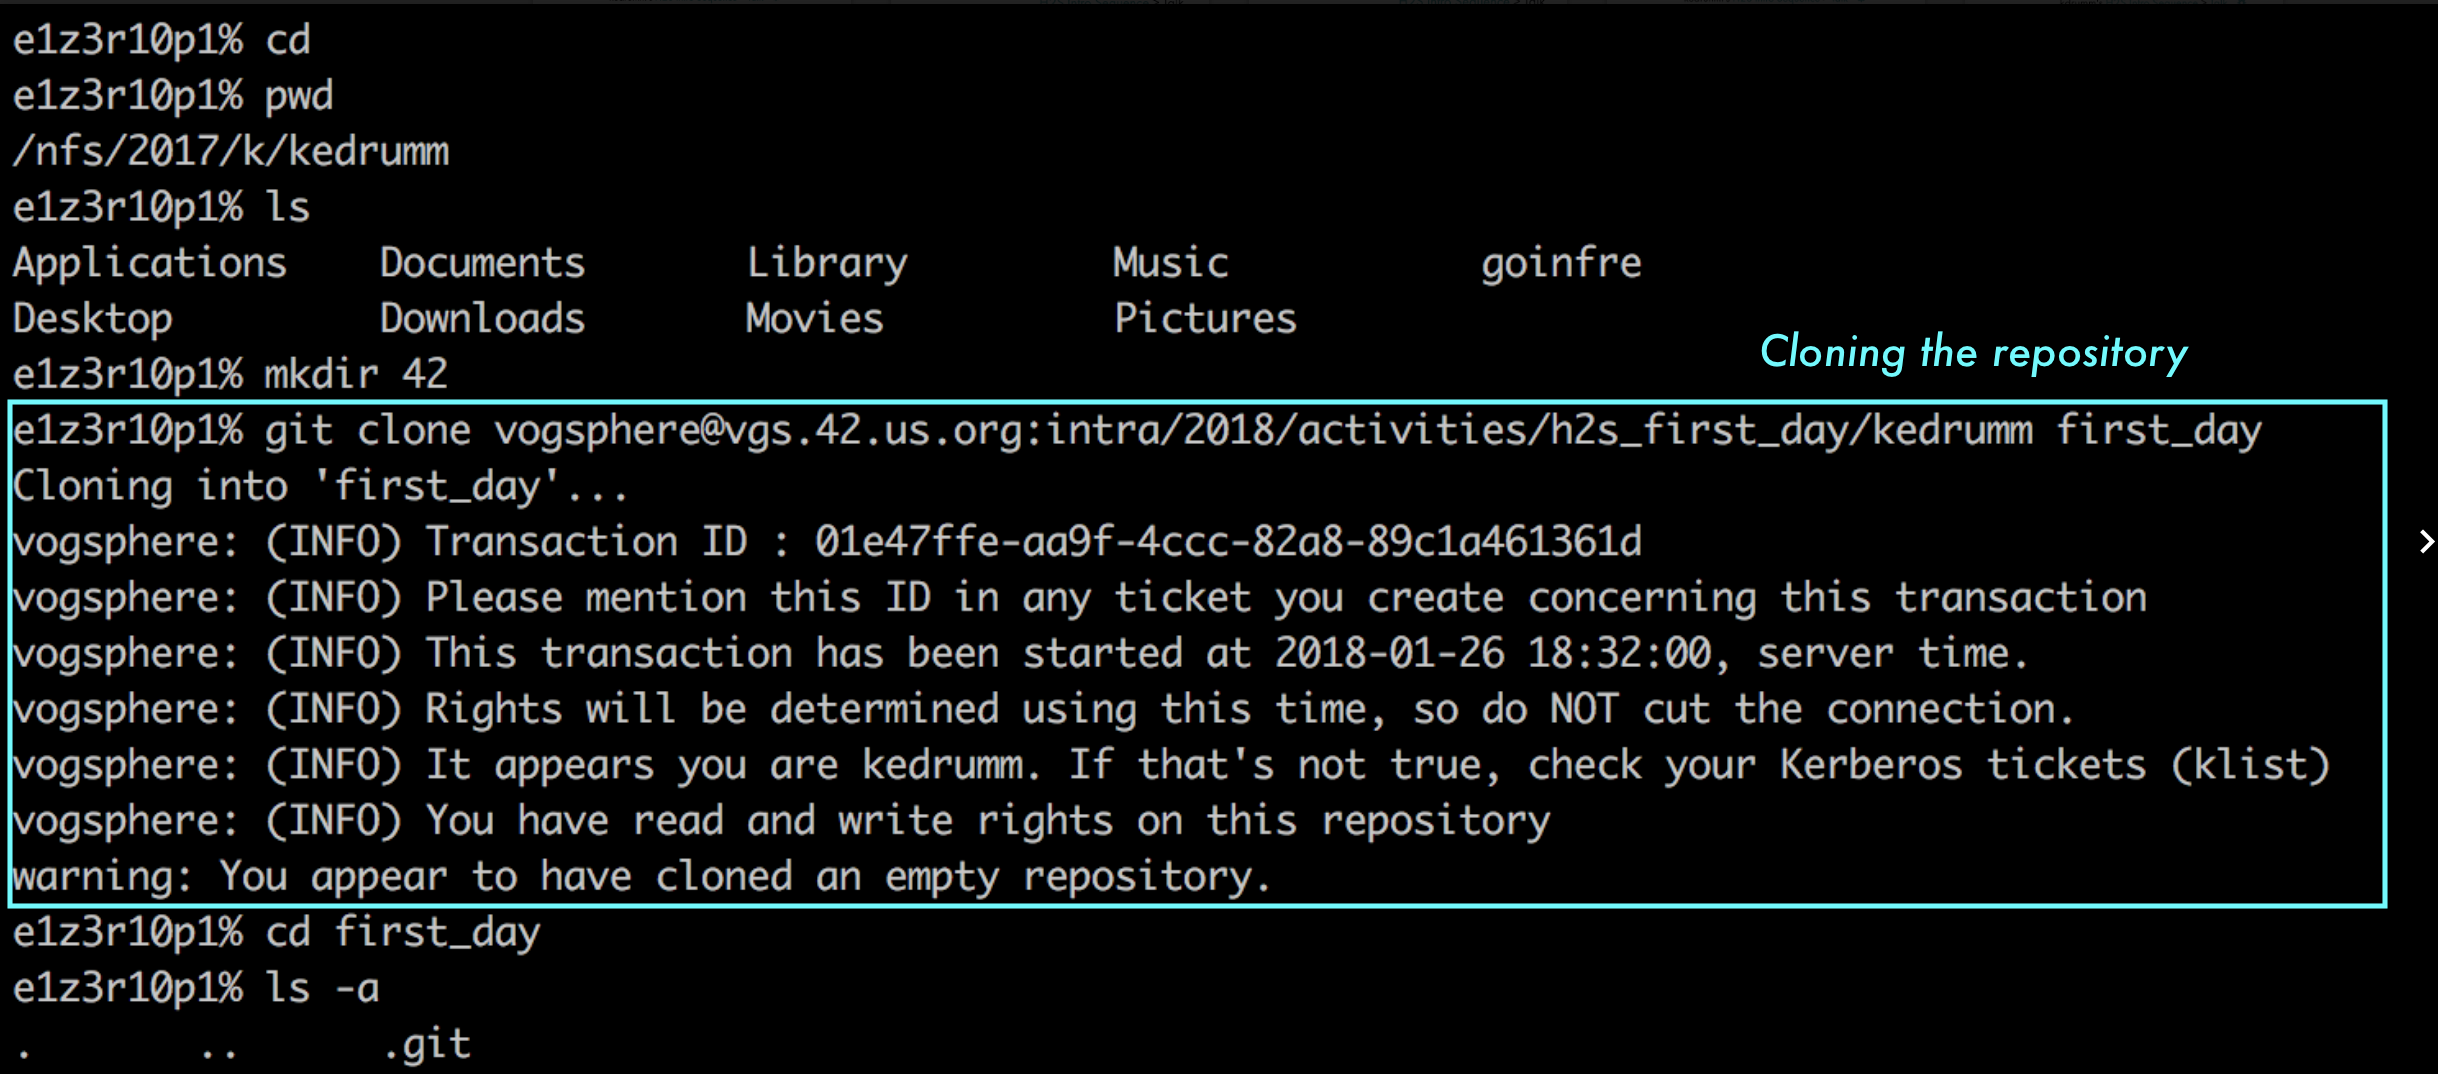
\includegraphics[width=1\textwidth]{screenshots/clone_first_day}

\hint{If you have an error during the git clone type "kinit <username>" and press enter. Then, type your intra password.}

%******************************************************************************%
%                                                                              %
%                                     Warmup                                   %
%                                                                              %
%******************************************************************************%

\chapter{Warmup before coding}

Here is the assignment for today - it is very simple. Look for a beginner's guide on command line navigation to help you find out how to do these things. Recommended: Michael Hartl's \href{https://www.learnenough.com/command-line-tutorial}{"Learn Enough Command Line to be Dangerous"}.


\begin{itemize}

	\item Create two folders inside the FirstDay project folder: dreams\_and\_visions and scholastic\_enterprises.
	\item Inside dreams\_and\_visions, create a text file (.txt). In the text file write a few sentences about what kind of coding you want to learn the most. For example, we have some projects to create interactive websites; some to create playable games; some to visualize math concepts and learn cryptography; a few coming with machine learning techniques; and one cool project to synthesize music.
	\item Also inside dreams\_and\_visions, use Terminal to create a hidden text file that does not show up when you type "ls" but does show up when you type "ls -a". Not sure how to do this? Time for rumors. Ask around.
	\item Inside the hidden text file, write down a phrase that is your favorite kind of compliment you like to receive.
	\item Use \texttt{chmod} to change the permissions of the hidden text file so that it is read-only for everybody, including yourself! Don't worry you can change it back later. Type "man chmod" at the terminal to learn about the needed command, or Google it.
	\item The permissions will change back to default when you submit your files to Vogsphere. Inside scholastic\_enterprises, Create a text file and write down your notes on chmod for reference later.

\end{itemize}

When done, use the instructions on the next page to turn in your work.

%******************************************************************************%
%                                                                              %
%                               Turning In Your Code                           %
%                                                                              %
%******************************************************************************%

\chapter{Turning in your code}

Turn in your work by typing three commands in order:
	\begin{itemize}
		\item git add *
		\item git commit -m "Today I worked on ..<your comments here>.."
		\item git push
	\end{itemize}
	\hint{Make sure you are in your project's git folder when you type the git add, git commit, git push commands.}
	\warn{If you have an error during the git push, you may need to refresh your authentication ticket. Do this by typing "kinit <username>" and then typing your intra password.}

Back on Intra, you can press the button "Set the Project as Finished" to indicate that you are ready for corrections.

	\hint{Pushing to Vogsphere more often is one way of saving your work.}

%******************************************************************************%
%                                                                              %
%                                 Corrections                                  %
%                                                                              %
%******************************************************************************%

\chapter{Corrections}
\begin{itemize}
	\item On your project page, click the button "Subscribe to Defense." Choose a time slot from the screen that shows next.

	\item When the appointment time comes, look up your assigned corrector on Slack and send them a message. Find each other.

	\item Corrector, sit at the correctee's station and open a new web browser in Incognito mode. Log into your intra.

	\item Access the corrections page. Clone their Git repository into a new folder.

	\item Click "Begin correction" and follow the instructions on the correction page.

	\item Use this time to chat about the project and the rest of your life.

	\item Once the correction is finished, your corrector should remember to log out of Intra.

	\item After both the correction is complete, in order to finalize your score you must then provide feedback for the corrector on your project page. Go to your project page and click the "feedback" button for each completed correction.

\end{itemize}

%******************************************************************************%
%                                                                              %
%                                 What's next?                                 %
%                                                                              %
%******************************************************************************%

\chapter{What's next?}

If you have extra time, here are a few things to do:

\begin{enumerate}
	\item Talk to your mentor about your previous coding experience and ask them for a challenging project to start with if you already know the basics of how to code in Ruby or Python, or if you want to work in a different programming language.

	\item Learn more about the command line, and Emacs or Vim.

	\item Learn more about the Git protocol and set up your own Github or Bitbucket account to save your code for yourself online.

	\item As always, you can move on to starting the next project right away. Beginners go to \href{https://projects.intra.42.fr/projects/h2s-intro-sequence}{H2S Intro Sequence.}

\end{enumerate}

%******************************************************************************%
%                                                                              %
%                               End of document                                %
%                                                                              %
%******************************************************************************%

\end{document}

